\section{Analysephase}

\begin{wrapfigure}[11]{r}[0cm]{170px}
	\vspace{-12px}
	\centering
	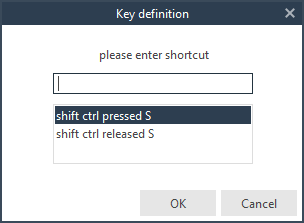
\includegraphics[width=170px]{../graphic/images/screenshots/Alter-Editor}
	\caption{Bestehender Editor}
	\label{fig:existEditor}
\end{wrapfigure}

\subsection{Ist-Analyse}

Seit früheren Versionen existierte bereits ein Editor zur Eingabe von Shortcuts (siehe \autoref{fig:existEditor}). Dieser ist allerdings sehr einfach aufgebaut und beschränkt sich auf die Eingabe eines Shortcuts per Tastatur. Außerdem ist es nicht möglich Warnungen anzuzeigen oder zwischen bestehenden Shortcuts zu navigieren. Da dieser Editor in keinerlei Hinsicht den gegebenen Anforderungen dieses Projekts entspricht, wurde eine Weiterentwicklung dessen vom Autor als nicht sinnvoll erachtet.

Die Funktionen, welchen Shortcuts zugeordnet werden sollen sind im ADITO Designer schon vorhanden. Zudem existieren sogenannte Entitys, welche Dateneinheiten darstellen und eben genannte Funktionen besitzen können. Beispielsweiße könnte ein Entity \glqq Person\grqq\xspace existieren, welche wiederum die Funktion \glqq Person hinzufügen\grqq\xspace besitzt. Dieser Funktion könnte nun ein Shortcut zugewiesen werden z.B. Strg + Einfg.

\subsection{Sollkonzept}

Der neue Editor muss ebenfalls die Eingabe aber auch die Bearbeitung (z.B. Entfernen einer einzelnen Taste) eines Shortcuts per Tastatur und Maus unterstützen. Für die Navigation und für einen besseren Überblick, werden alle bestehenden Tastenkombinationen in tabellarischen Form präsentiert. Es soll zu jedem Zeitpunkt ersichtlich sein, für welche Funktion der Shortcut definiert wird. Eine weitere Anforderung besteht darin, alle Warnungen für die entsprechenden Browser und deren Betriebssysteme anzuzeigen.

\subsection{Anwendungsfälle}

Um eine grobe Übersicht über alle Anwendungsfälle zu erhalten, die von dem umzusetzenden Editor
abgedeckt werden sollen, wurde im Laufe der Analysephase ein Use-Case-Diagramm erstellt. Dieses
Diagramm befindet sich im Anhang \autoref{fig:anwendungsfall} auf \autopageref{fig:anwendungsfall}.

\subsection{\glqq Make or Buy\grqq -Entscheidung}
Die Entscheidung, ob der Editor selber erstellt oder gekauft werden soll, lässt sich einfach treffen. Sucht man auf dem Markt nach Softwareteilen, welche den Anforderungen dieses Projekts genüge tun, so findet man nichts entsprechendes. Darum ist man gewissermaßen gezwungen den Editor selbst zu erstellen.

\newpage
